\documentclass{article}

\usepackage{xeCJK}
\setCJKmainfont{SimSun}
\usepackage{hyperref}
\usepackage{listings}
\lstset{breaklines}



\title{Report of Course: FPGA-based Digital System Design}
\author{李约瀚 \\ 14130140331 \\ qinka@live.com \\ me@qinka.pro}



\begin{document}

\maketitle
\newpage
\tableofcontents
\newpage

\section{Summary}
\label{sec:summary}

In this report, I talked about the microprocessor Parwan,
and instance one of the component(alu) in the data section.
Meanwhile, there are also the behavior simulation and post-route simulation.


\section{Parwan Processor}
\label{sec:parwan}

Parwan processor is a 8-bit microprocessor, which is more suitable for those who want to learn about microprocessor.
Though Parwan is not just like Intel's 8051 which can be used in industry to controlling some things,
the architecture and design of Parwan is worth learning. 
It's hard to find the beginning and history of Parwan on the Internet, so this part will be skipped.

The width of address bus of 8-bit processor, Parwan is 12 bits.The first four highest bits of bus are id of page,
and the others are the offset. The maximum size of memory is 4096 bytes. Meanwhile, there is a data bus, connected with memory.

There are totally 17 commands in the Parwan, including 6 full address commands, 5 page address commands, and 6 no address commands.
For the full address commands, the first four lower bits in command is the id of page, while fifth bit of command controls
the addressing in whether direct way of indirect way. As the commands can be classified by function, jumping for example,
classifying by address can make easier to design the binary code of command.

Parwan includes data section and control section. The alu, ac, shu, sr, ir, pc, and mar are belong to data section,
while the function of control section is operating those in data section.
The control section is driven by state machine.

\section{Instance of ALU}
\label{sec:alu}

In this section, I will try to instance ALU. Then test and simulate it.

\subsection{Instance}
\label{sec:alu:instance}

The following is the VHDL codes of the ALU.

\begin{lstlisting}[language=VHDL]
library IEEE;
use IEEE.STD_LOGIC_1164.ALL;
entity alu is
    port( a_side, b_side : in STD_LOGIC_VECTOR(7 downto 0);
          alu_out : out STD_LOGIC_VECTOR(7 downto 0);
          alu_a, alu_b, alu_and, alu_not, alu_add, alu_sub : in STD_LOGIC;
          in_flags : in STD_LOGIC_VECTOR(3 downto 0);
          out_flags : out STD_LOGIC_VECTOR(3 downto 0)
          );
end alu;

architecture Behavioral of alu is
begin
    process(a_side,b_side,alu_and,alu_not,alu_a,alu_b,alu_add,alu_sub)
        variable t : STD_LOGIC_VECTOR(9 downto 0) := "0000000000";
        variable fv,fc,fz,fn : STD_LOGIC;
        alias v_flag_in : STD_LOGIC is in_flags(3);
        alias c_flag_in : STD_LOGIC is in_flags(2);
        alias z_flag_in : STD_LOGIC is in_flags(1);
        alias n_flag_in : STD_LOGIC is in_flags(0);
    -- for add' cv
        variable c : STD_LOGIC_VECTOR(9 downto 0);
        variable a_sign, b_sign : STD_LOGIC;
    -- a side, b_side
        variable a,b : STD_LOGIC_VECTOR(7 downto 0);
    begin
        case STD_LOGIC_VECTOR'(alu_and,alu_sub,alu_and,alu_not,alu_a,alu_b) is
            -- add
            when "100000" =>
                a := a_side;
                b := b_side;
                a_sign := a(7);
                b_sign := b(7);
                t(0) := a(0) xor b(0) xor c_flag_in;
                c(0) := ((a(0) xor b(0)) and c_flag_in) or (a(0) and b(0));
                for i in 1 to 7 loop
                    t(i) := a(i) xor b(i) xor c(i-1);
                    c(i) := ((a(i) xor b(i)) and c(i-1)) or (a(i) and b(i));
                end loop;
                t(8) := c(7);
                if (a_sign = b_sign) and (t(7) /= a_sign) then
                    t(9) := '1'; -- means overflow
                else
                    t(9) := '0';
                end if;
                fc := t(8);
                fv := t(9);
            -- sub
            when "010000" =>
                a :=     a_side;
                b := not b_side;
                a_sign := a(7);
                b_sign := b(7);
                t(0) := a(0) xor b(0) xor (not c_flag_in);
                c(0) := ((a(0) xor b(0)) and (not c_flag_in)) or (a(0) and b(0));
                for i in 1 to 7 loop
                    t(i) := a(i) xor b(i) xor c(i-1);
                    c(i) := ((a(i) xor b(i)) and c(i-1)) or (a(i) and b(i));
                end loop;
                t(8) := c(7);
                if (a_sign = b_sign) and (t(7) /= a_sign) then
                    t(9) := '1'; -- means overflow
                else
                    t(9) := '0';
                end if;
                fc := t(8);
                fv := t(9);
            -- and
            when "001000" =>
                t(7 downto 0) := a_side and b_side;
                fc := c_flag_in;
                fv := v_flag_in;
            -- or
            when "000100" =>				
                t(7 downto 0) := not b_side;
                fc := c_flag_in;
                fv := v_flag_in;
            -- a
            when "000010" =>
                t(7 downto 0) := a_side;
                fc := c_flag_in;
                fv := v_flag_in;
            -- b
            when "000001" =>
                t( 7downto 0) := b_side;				
                fc := c_flag_in;
                fv := v_flag_in;
            -- null
            when others => null;
        end case;
        fn := t(7);
        if t(7 downto 0) = "0000000" then
            fz := '1';
        else
            fz := '0';
        end if;
        alu_out <= t(7 downto 0);
        out_flags <= (fv,fc,fz,fn);
    end process;	
end Behavioral;
\end{lstlisting}

\subsection{Behavior Simulation}
\label{sec:alu:b-sim}

After instancing ALU, the behavior simulation will be done.

The following is the codes about test bench.

\begin{lstlisting}[language=VHDL]
LIBRARY ieee;
USE ieee.std_logic_1164.ALL;
USE ieee.std_logic_unsigned.ALL;
ENTITY alu_test IS
END alu_test;

ARCHITECTURE behavior OF alu_test IS
    COMPONENT alu
        PORT(
            a_side : IN  std_logic_vector(7 downto 0);
            b_side : IN  std_logic_vector(7 downto 0);
            alu_out : OUT  std_logic_vector(7 downto 0);
            alu_a : IN  std_logic;
            alu_b : IN  std_logic;
            alu_and : IN  std_logic;
            alu_not : IN  std_logic;
            alu_add : IN  std_logic;
            alu_sub : IN  std_logic;
            in_flags : IN  std_logic_vector(3 downto 0);
            out_flags : OUT  std_logic_vector(3 downto 0)
        );
    END COMPONENT;    
    signal a_side : std_logic_vector(7 downto 0) := (others => '0');
    signal b_side : std_logic_vector(7 downto 0) := (others => '0');
    signal alu_a : std_logic := '0';
    signal alu_b : std_logic := '0';
    signal alu_and : std_logic := '0';
    signal alu_not : std_logic := '0';
    signal alu_add : std_logic := '0';
    signal alu_sub : std_logic := '0';
    signal in_flags : std_logic_vector(3 downto 0) := (others => '0');    
    signal alu_out : std_logic_vector(7 downto 0);
    signal out_flags : std_logic_vector(3 downto 0);    
    signal ops : std_logic_vector(5 downto 0):= "000001";
    signal flags : std_logic_vector(3 downto 0) := "0000";
    signal va : std_logic_vector(7 downto 0):= "00000000";
    signal vb : std_logic_vector(7 downto 0):= "00000000";
    constant clk_period : time := 100 ns;    
BEGIN
    a_side <= va;
    b_side <= vb;
    alu_a <= ops(0);
    alu_b <= ops(1);
    alu_and <= ops(2);
    alu_not <= ops(3);
    alu_add <= ops(4);
    alu_sub <= ops(5);
    in_flags <= flags;
    uut: alu PORT MAP (
        a_side => a_side,
        b_side => b_side,
        alu_out => alu_out,
        alu_a => alu_a,
        alu_b => alu_b,
        alu_and => alu_and,
        alu_not => alu_not,
        alu_add => alu_add,
        alu_sub => alu_sub,
        in_flags => in_flags,
        out_flags => out_flags
        );
    clk_process :process
    begin
        wait for clk_period/2;
        flags <= flags + 1;
        if flags = "0000" then
            ops <= ops(4 downto 0) & ops(5);
        end if;
    end process;
    stim_proc: process
    begin
        va <= "01011010";
        vb <= "00001111";    
        wait;
    end process;
END;
\end{lstlisting}
 
The figure \ref{fig:cr-1} and the figure \ref{fig:cr-2} is the result of the behavior simulation. 
 
\begin{figure}
\centering
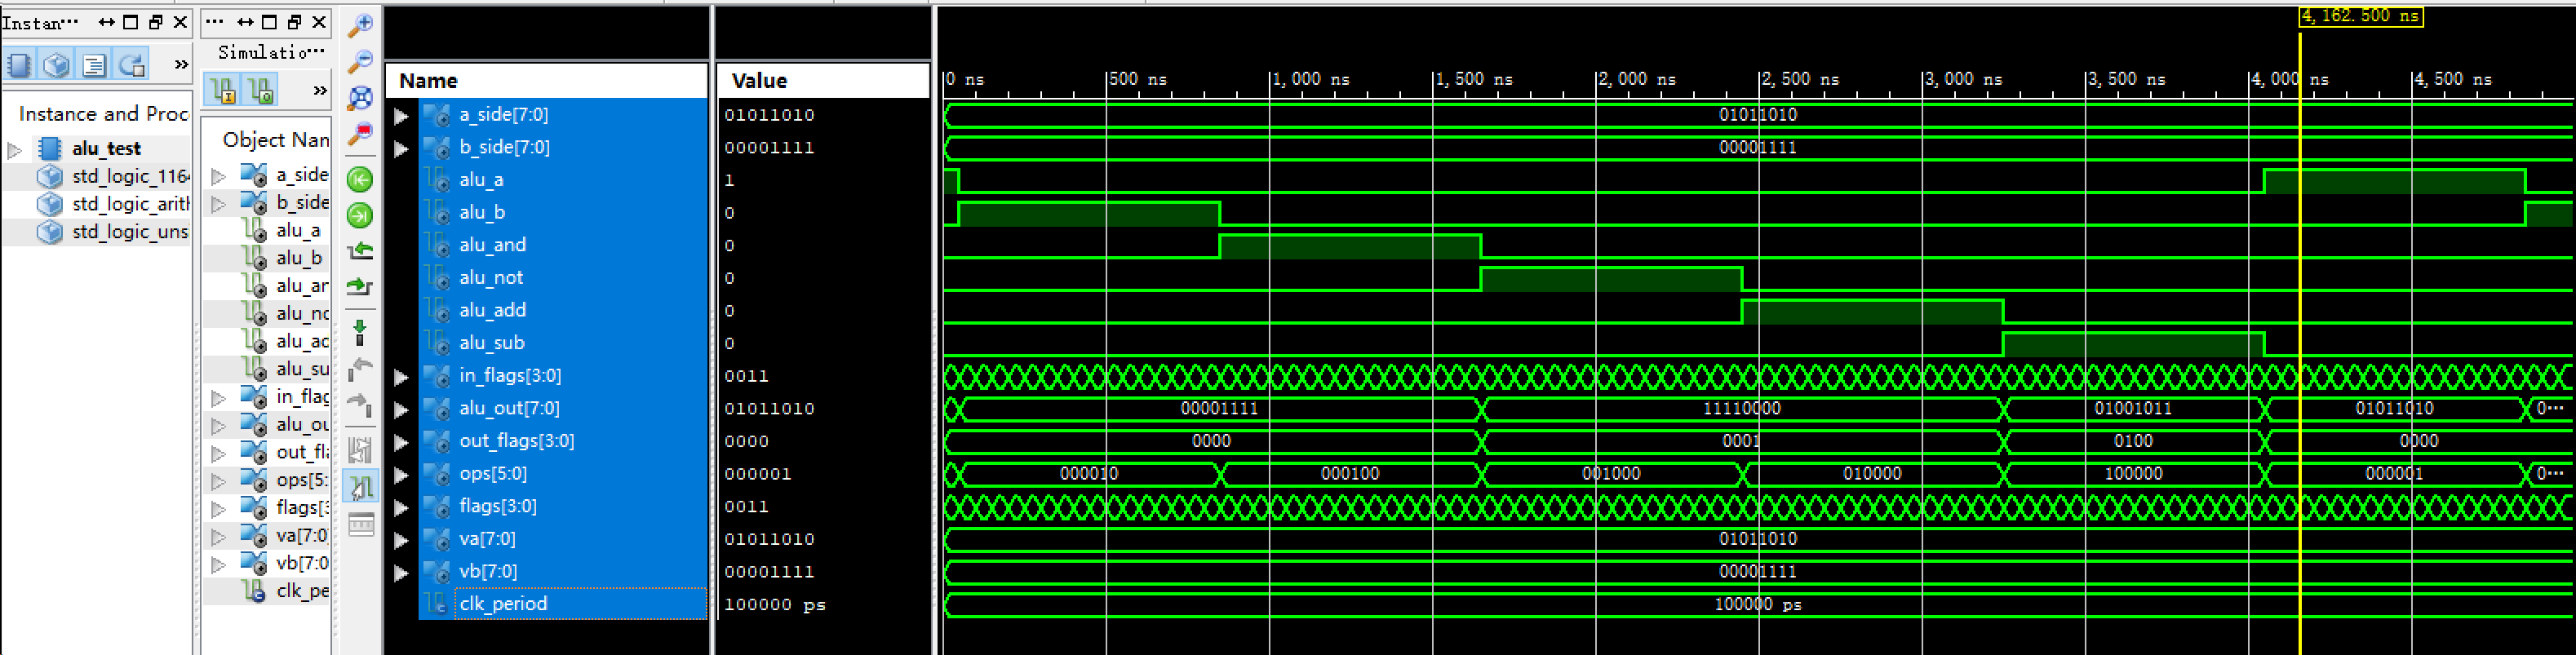
\includegraphics[width=0.7\linewidth]{cr-1}
\caption{The result of behavior simulation.}
\label{fig:cr-1}
\end{figure}

\begin{figure}
\centering
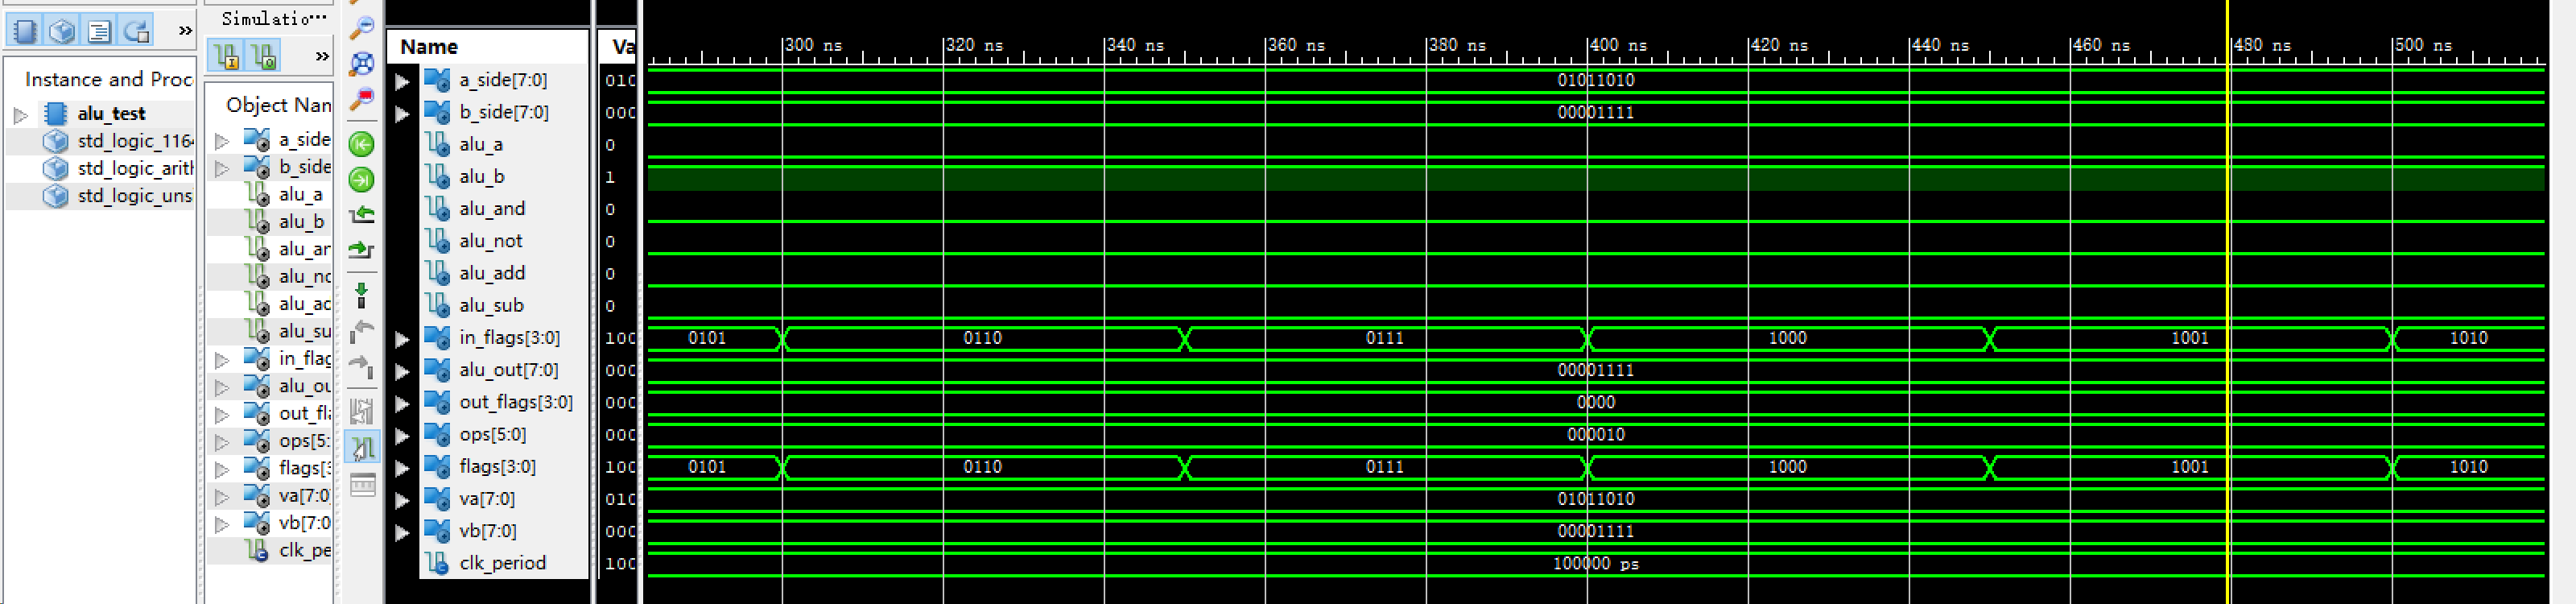
\includegraphics[width=0.7\linewidth]{cr-2}
\caption{The detail of the result of behavior l}
\label{fig:cr-2}
\end{figure}

And in the behavior simulation, the alu work well.


\subsection{Post-route Simulation}
\label{sec:alu:p-sim}

This section is about the post-route simulation. The codes of test bench is the one of behavior simulation.

\begin{figure}
\centering
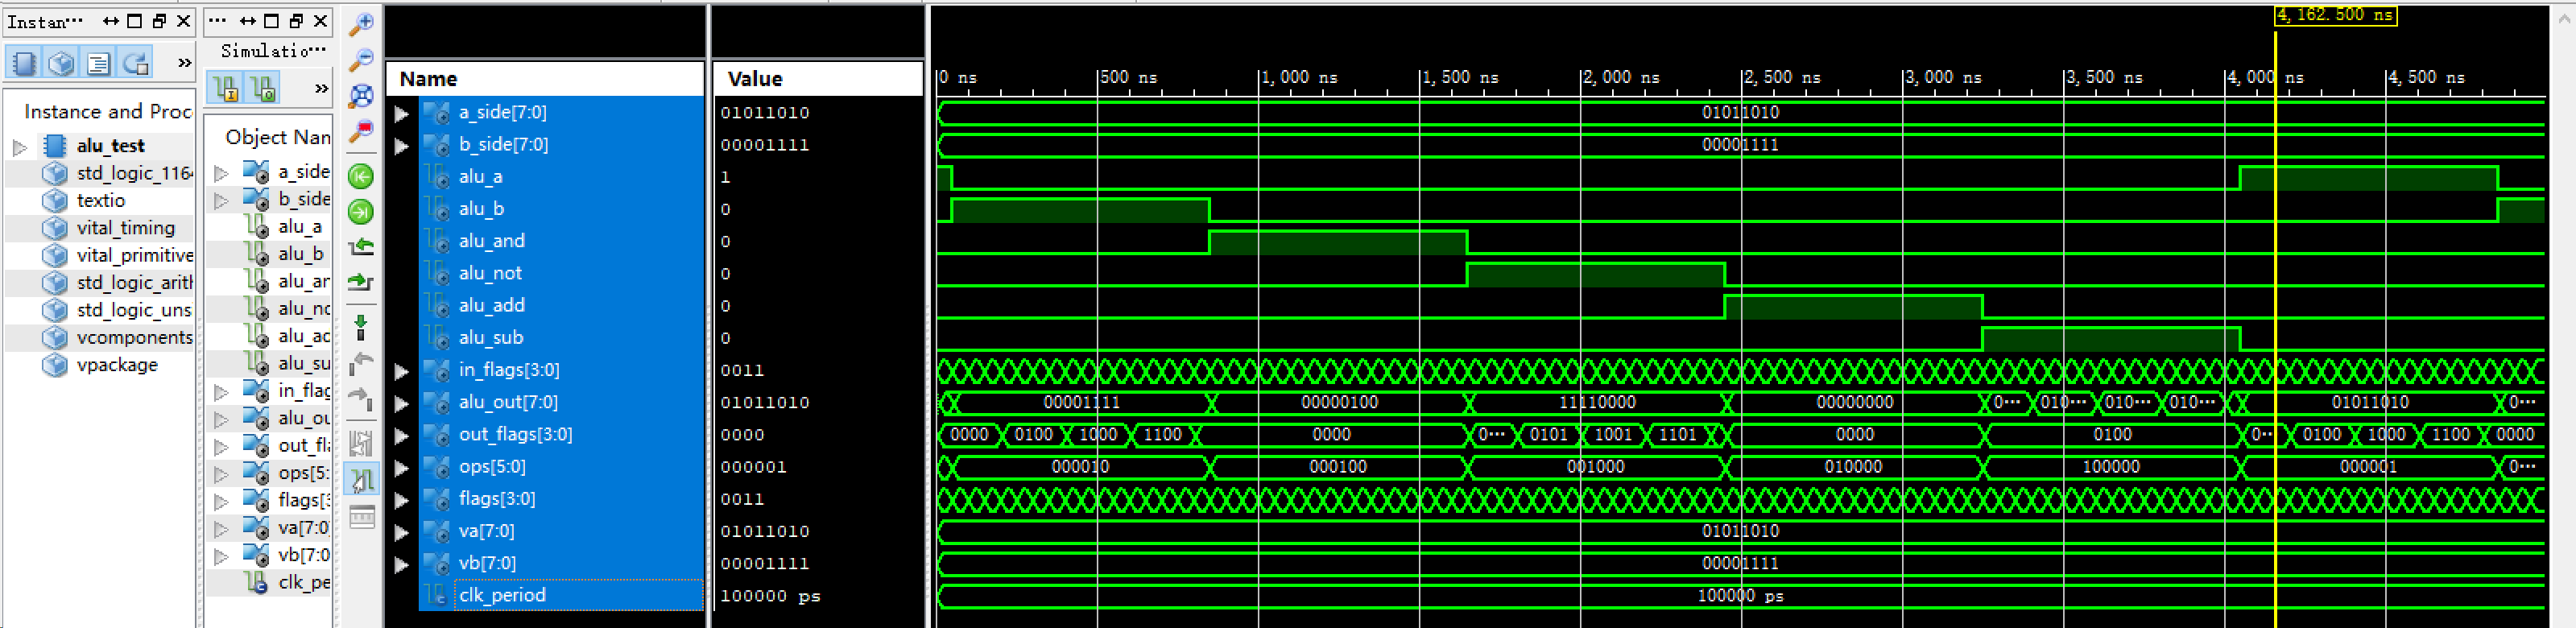
\includegraphics[width=0.7\linewidth]{cr-3}
\caption{The result of post-route simulation.}
\label{fig:cr-3}
\end{figure}

\begin{figure}
\centering
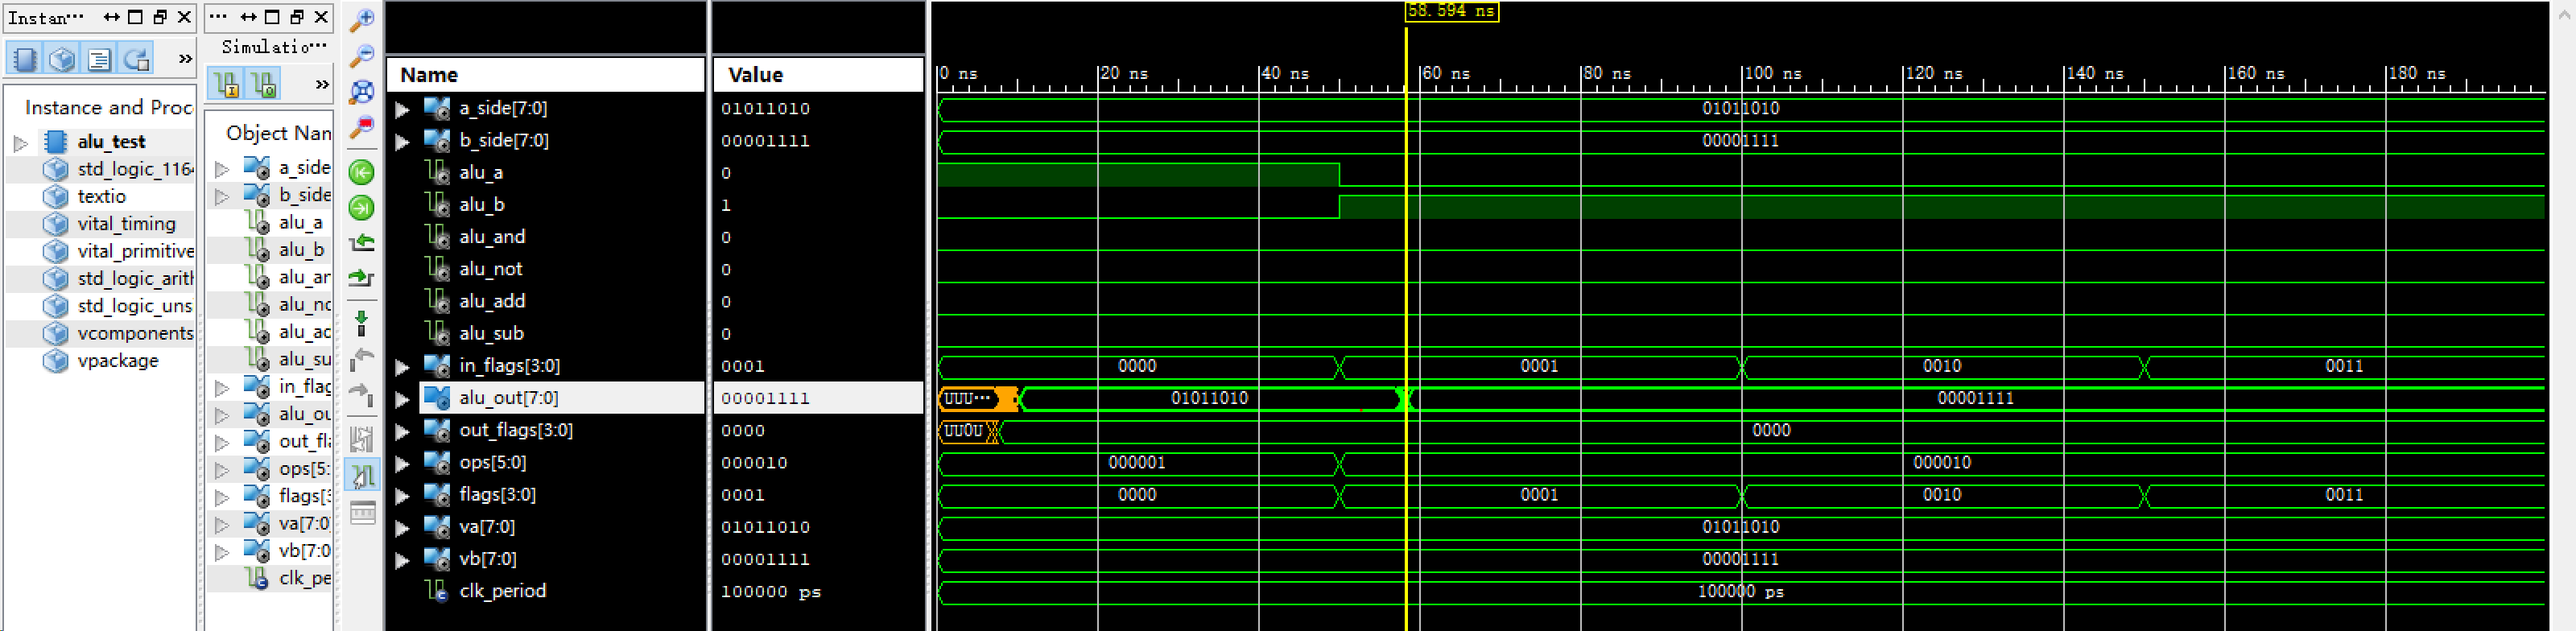
\includegraphics[width=0.7\linewidth]{cr-4}
\caption{The detail of post-route simulation's result.}
\label{fig:cr-4}
\end{figure}

The results of post-route simulation are in the figure \ref{fig:cr-3}, and figure \ref{fig:cr-4}.
The delay in the circuit\footnote{That delay means the delay between ``input'' and ``output''.} is about 8 ns.
So the maximum of the frequency of the circuit is about 116.3MHz, and the 50MHz might be a good frequency might a good choice.


\end{document}